\section{Overview}







图 \ref{Overview} 是BAN(Body Area Network)的构想图,假设了三个设备在BAN 上的情况。



\begin{figure*}[htbp]
\begin{center}
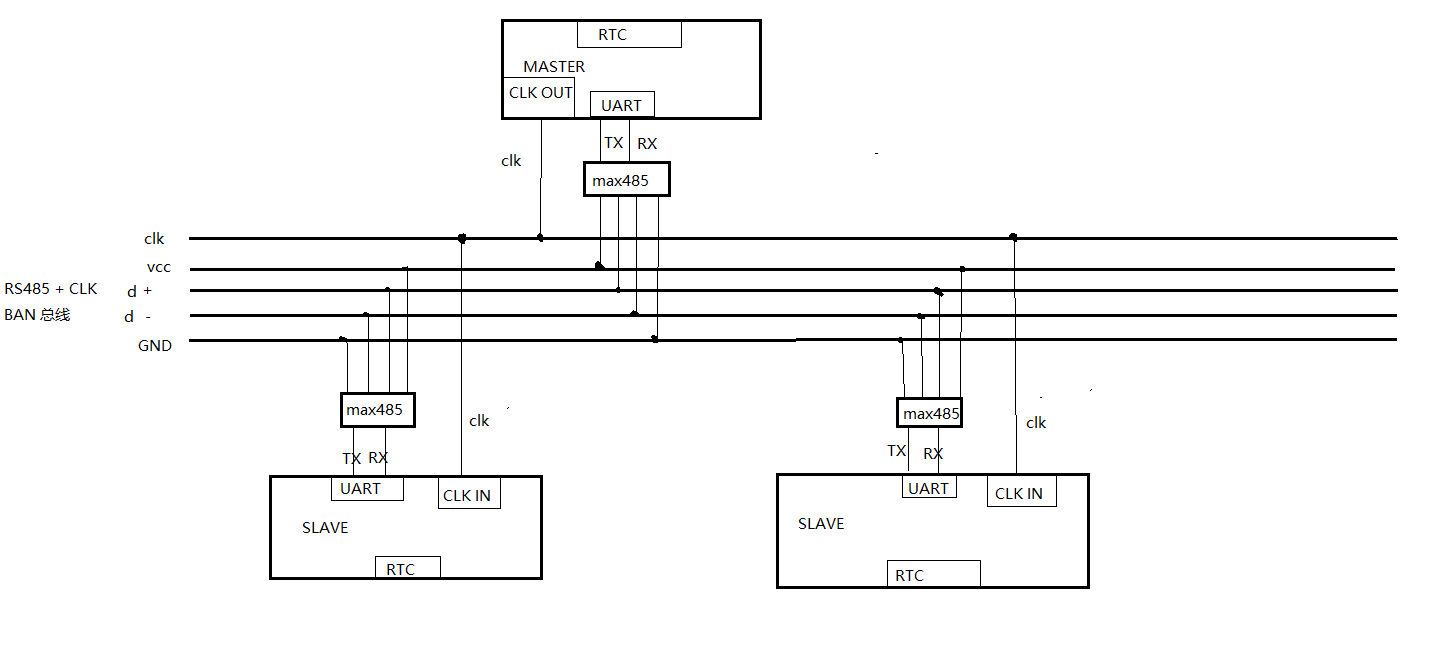
\includegraphics[width=15cm]{img/overview}
\caption{BAN }
\label{Overview}
\end{center}
\vspace{-0.5em}
\end{figure*}


下面是对于这个构想图模块的解释。




\subsection{CLK}

这个是BAN 的时钟线,时钟信号由 MASTER 产生,挂载在总线上的从设备会去监测捕获这条时钟线
的上升沿。时钟的产生方式是:定时器产生的PWM。如图\ref{timer} \tikz \fill[red] (1ex,1ex) circle (1ex);

\begin{figure*}[htbp]
\begin{center}
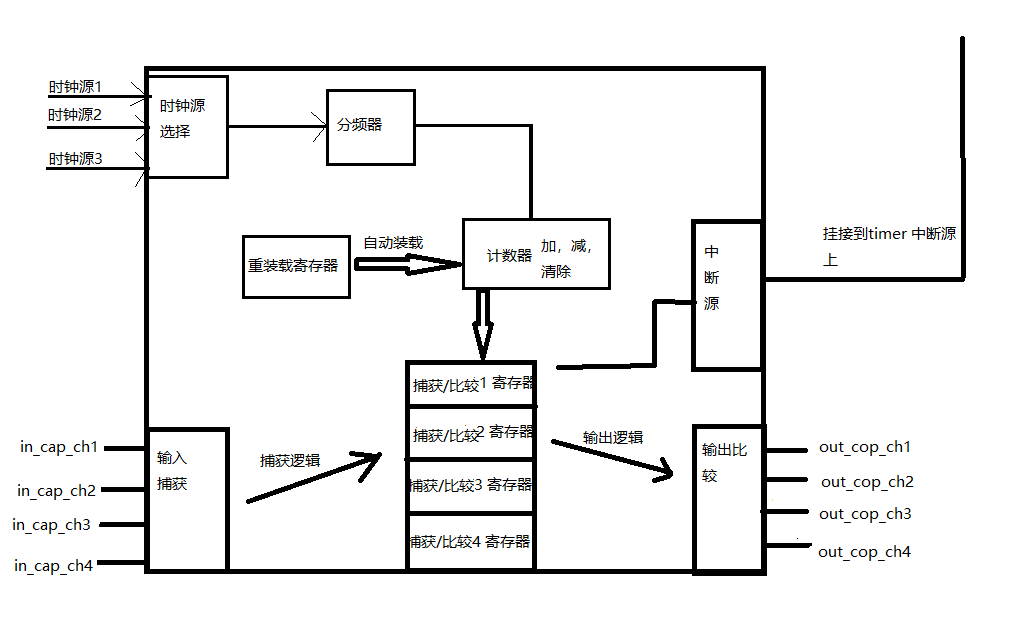
\includegraphics[width=15cm]{img/timer}
\caption{PWM}
\label{timer}
\end{center}
\vspace{-0.5em}
\end{figure*}






\subsection{RTC}

大多数时候RTC 其实是一个独立供电的(纽扣电池),有特殊寄存器(年月日)的 timer。

在本次测试中,由于时间和硬件资源的原因,每一个设备都会使用一个精准定时器用于精确
定时,维护一个unsigned long long 类型的时间戳。

\begin{figure*}[htbp]
  
\begin{tikzpicture}
\draw (0,0) -- (1,0) -- (1,1) -- cycle;
  \end{tikzpicture}
\caption{Do not forget!}
\end{figure*}



\subsection{UART}
